% !TeX spellcheck = fr_FR
% !TeX spellcheck = fr_FR
%%%%%%%%%%%%%%%%%%%%%%%%%%%%%%%%%%%%%%%%%%%%%%%%%%%%%%%%%%%%%%%%%%%%%%%%%%%%%%%%
%%                                                                             %
%% HEPIA BACHELOR ABSTRACT LATEX TEMPLATE                                      %
%% version 0.10 - 2020/04/25                                                    %                                                                             %
%%                                                                             %
%%%%%%%%%%%%%%%%%%%%%%%%%%%%%%%%%%%%%%%%%%%%%%%%%%%%%%%%%%%%%%%%%%%%%%%%%%%%%%%%


%% To fill up by the student
% \newcommand{\Session}{Printemps 2020}
% \newcommand{\Author}{}
% \newcommand{\Professor}{< Pr\'enom NOM >}
% \newcommand{\Client}{< Pr\'enom NOM >}
\newcommand{\Convention}{non}
\newcommand{\Confidentiel}{non}

\documentclass[12pt]
			{report}	% Set document to report class
\usepackage[T1]
			{fontenc}	% Font enconding
\usepackage[utf8]
			{inputenc}	% Set input encoding to utf-8, thus allow for non-ASCII characters
\usepackage[french]
			{babel}		% set document to default language to french
\usepackage[cm]
			{fullpage}	% Set margins to full page
\usepackage[a4paper,includehead,headheight=24pt,left=2.5cm, right=2.5cm, bottom=2.5cm, top=1.26cm]
			{geometry}	% Configure document geometry

\usepackage{tikz}		% Image and drawing related package
\usepackage{helvet}		% Helvetica font ~ Arial
\usepackage{mathptmx}	% Times font ~ Times New Roman


\usepackage[sfmath,notextcomp]{kpfonts} % Calibri replacement, font is \sf

\usepackage[scaled=0.85]
			{beramono}	% Vera mononspace {fvm}
\usepackage	{berasans}	% Vera sans {fvs}

%% This defines the default sans serif, roman and monospace fonts
\renewcommand{\sfdefault}
				{phv}	% helvetica as sans serif font
\renewcommand{\rmdefault}
				{ptm}	% times as roman (serif) font
\renewcommand{\ttdefault}
				{fvm}	% Vera mononspace as monospace font
\usepackage{bold-extra}	% Allow custom typsettings horrors like bold Small Caps
\usepackage{slantsc}	% Allow custom typsettings horrors like slanted Small Caps
\usepackage{numprint}	% number notation related package, e.g 10'000'000
\usepackage{setspace}	% linespacing related package


\usepackage{lipsum}		% Lorem Ipsum generator
%\usepackage{showframe}	% Print document frame


%%%%%%%%%%%%%%%%%%%%%%%%%%%%%%%%%%%% CUSTOM HEADER %%%%%%%%%%%%%%%%%%%%%%%%%%%%%
\usepackage{fancyhdr}
\pagestyle{fancy}
\renewcommand{\headrulewidth}{0pt}
\fancyhf{}
\fancypagestyle{plain}{
	\fancyhf{}%
	\fancyhead[L,C]{}
	\fancyhead[R]{\fontsize{11pt}{12.4pt} \sf \textbf{\\*\Session\\*[1.2pt]Session de bachelor}}
	\fancyfoot[L,C,R]{}
	\renewcommand{\headrulewidth}{0pt}
	\renewcommand{\footrulewidth}{0pt}
}
%%%%%%%%%%%%%%%%%%%%%%%%%%%%%%%% CUSTOM CHAPTER TITLES %%%%%%%%%%%%%%%%%%%%%%%%%
\usepackage{titlesec}
\titleformat{\chapter}[hang]{\centering \bfseries\scshape\Large}{\thechapter.}{1pc}{}
\titleformat{name=\chapter,numberless}[hang]{\fontsize{15.5}{18.7}\centering\bfseries\scshape}{}{1pc}{}
\titlespacing{\chapter}{0pt}{3em}{-12pt}
%\usepackage{showframe}	% Prints document frame

%%%%%%%%%%%%%%%%%%%%%%%%%%%%%%%%%%%%%%%%%%%%%%%%%%%%%%%%%%%%%%%%%%%%%%%%%%%%%%%%
%%%%%%%%%%%%%%%%%%%%%%%%%%%%%%%% DOCUMENT STARTS BELOW %%%%%%%%%%%%%%%%%%%%%%%%%
%%%%%%%%%%%%%%%%%%%%%%%%%%%%%%%%%%%%%%%%%%%%%%%%%%%%%%%%%%%%%%%%%%%%%%%%%%%%%%%%
\begin{document}
\chapter*{Résumé}
%% HEADER IMAGES
\tikz[remember picture,overlay] \node[shift={(4.655cm,-1.95cm)}] at (current page.north west)
{
\includegraphics[width=5.86cm,height=3.31cm]{template/images/title/hepia_logo}};
\begin{spacing}{0.956}
\vspace{0.5cm}

%% CONTENT STARTS HERE
Depuis l'antiquité à nos jours, les cartes sont le reflet des premières formes de données récoltées par l'Homme.
La cartographie a aidé l'humanité à définir des chemins à travers le monde et à naviguer.
Cependant avec les fortes avancées technologiques des dernières décennies, les données récoltées ont augmenté massivement et notablement dans la cartographie avec les données LIDAR. Elles représentent une des informations collectées des plus massives.
Elles sont utilisées dans l'étude topographique de régions, dans les géosciences, dans la science environnementale ou bien encore elles viennent en aide au guidage automatique de véhicule terrestre. Un problème fréquent lié à ces données est le traitement réalisé avant leurs utilisations dans des applications, qui est souvent nécessaire afin de filtrer tout ce qui ne présente aucune utilité et pourrait même fausser les résultats.
Il reste cependant difficile de les traiter manuellement due à la quantité de données importante. Pour ce faire, des méthodes analytiques sont employées afin d'accélérer ce processus au travers de systèmes automatisés.
Un autre problème présent est leurs utilisations pour reconstruire des surfaces. Les méthodes automatisées n'étant pas à 100\% fiables, il est nécessaire de vérifier la cohérence des données ainsi que la qualité des maillages produits. Ce travail se focalise sur principalement sur la création d'outils de traitement de données LIDAR et l'affichage de ces données au travers d'un client web. Il est également focalisé sur la conception d'outils de traitement de maillage résultant d'un traitement de données LIDAR.).


\vfill
\begin{center}
	{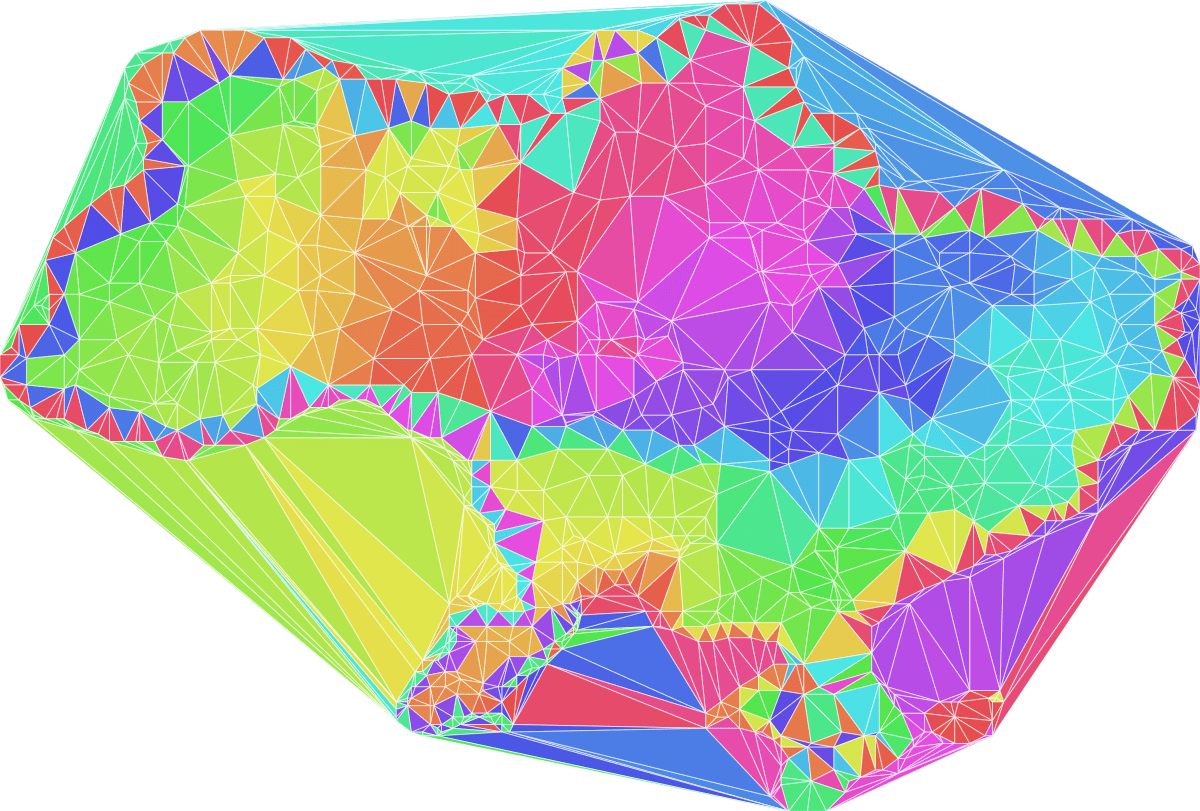
\includegraphics[width=280px]{figures/delaunator.png}}\\*
\vfill
%% CONTENT ENDS HERE



{
%%%%%%%%%%%%%%%%%%%%%%%%%%%%%%%%%%%%%%%%%%%%%%%%%%%%%%%%%%%%%%%%%%%%%%%%%%%%%%%%
%%%%%%%%%%%%%%%%%%%%%%%%%% DO NOT MODIFY THE TABLE BELOW %%%%%%%%%%%%%%%%%%%%%%%
%%%%%%%%%%%%%%%%%%%%%%%%%%%%%%%%%%%%%%%%%%%%%%%%%%%%%%%%%%%%%%%%%%%%%%%%%%%%%%%%
	\begin{tabular*}{16cm}{p{7.59cm} p{7.58cm}}
		\small Candidat-e:					&	\small Professeur-e(s) responsable(s):\\*[10pt]
		\small\textbf{\textsc{\Author}}		&	\small\textbf{\textsc{\Professor}}\\*[10pt]
		\footnotesize  Filière d’études : ITI %\textbf{En collaboration avec:} < Nom de l’entreprise >
		\footnotesize  {} & \footnotesize  Travail de bachelor soumis à une convention de stage en entreprise: \Convention\\*[20pt]
		\footnotesize  {} & \footnotesize  Travail soumis à un contrat de confidentialité: \Confidentiel\\*[10pt]
	\end{tabular*}\\*[1.9cm]
}

% \textit{Attention : le résumé doit impérativement tenir sur une seule page}

\end{center}
\end{spacing}
\end{document}          


% \thispagestyle{noheader}
% \chapter*{Résumé} % No (numbered) toc entry with *
% \addcontentsline{toc}{chapter}{Résumé} % Adding toc entry
% \thispagestyle{noheader}
% 
% Depuis l'antiquité à nos jours, les cartes sont le reflet des premières formes de données récoltées par l'Homme.
% La cartographie a aidé l'humanité à définir des chemins à travers le monde et à naviguer.
% Cependant avec les fortes avancées technologiques des dernières décennies, les données récoltées ont augmenté massivement et notablement dans la cartographie avec les données LIDAR. Elles représentent une des informations collectées des plus massives.
% Elles sont utilisées dans l'étude topographique de régions, dans les géosciences, dans la science environnementale ou bien encore elles viennent en aide au guidage automatique de véhicule terrestre. Un problème fréquent lié à ces données est le traitement réalisé avant leurs utilisations dans des applications, qui est souvent nécessaire afin de filtrer tout ce qui ne présente aucune utilité et pourrait même fausser les résultats.
% Il reste cependant difficile de les traiter manuellement due à la quantité de données importante. Pour ce faire, des méthodes analytiques sont employées afin d'accélérer ce processus au travers de systèmes automatisés.
% Un autre problème présent est leurs utilisations pour reconstruire des surfaces. Les méthodes automatisées n'étant pas à 100\% fiables, il est nécessaire de vérifier la cohérence des données ainsi que la qualité des maillages produits. Ce travail se focalise sur principalement sur la création d'outils de traitement de données LIDAR et l'affichage de ces données au travers d'un client web. Il est également focalisé sur la conception d'outils de traitement de maillage résultant d'un traitement de données LIDAR.
% 
% \begin{figure}[htbp!]
%     \centering
%     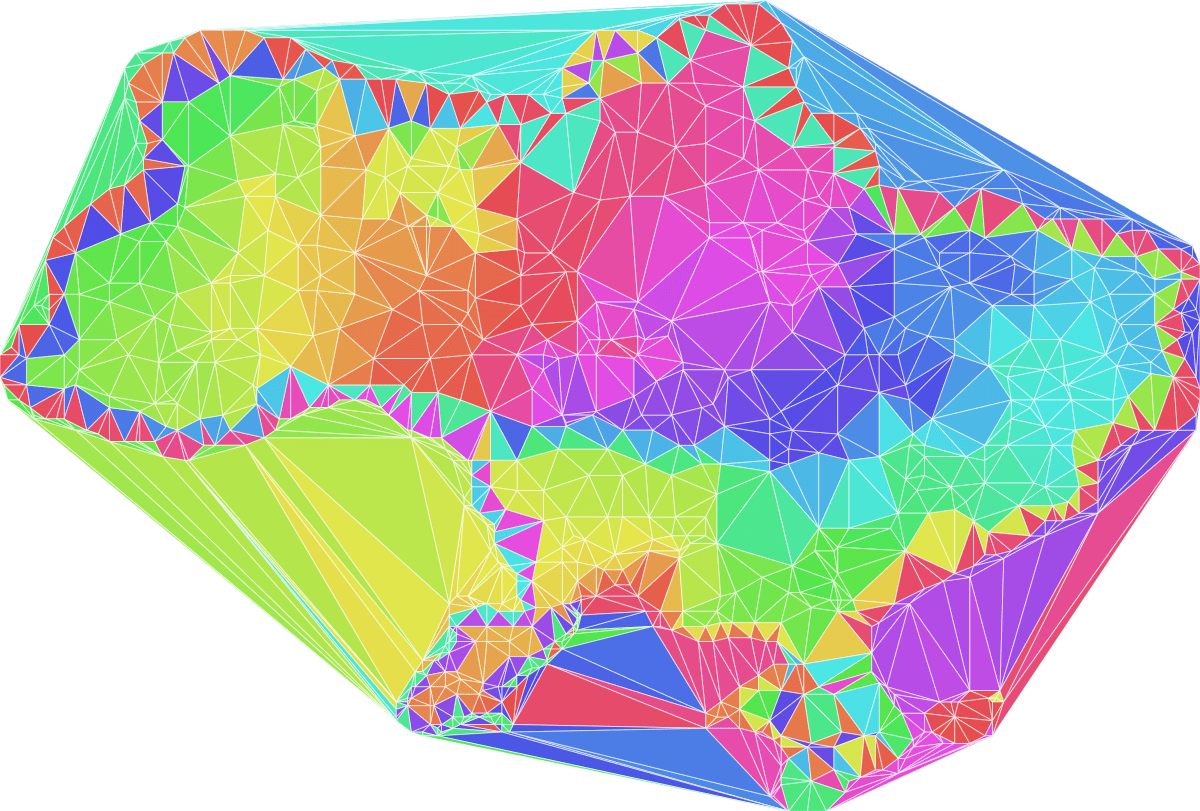
\includegraphics[width=0.2\linewidth]{figures/delaunator.png}
%     %\caption{Maillage résultant d'une triangulation de Delaunay. Source : tiré de \href{https://github.com/mapbox/delaunator}{https://github.com/mapbox/delaunator}}
%     %\label{fig:my_label}
% \end{figure}
% \begin{tabular*}{20cm}{>{\centering}m{7.59cm}>{\centering}m{7.58cm}}
% 	%% SUPERVISOR
% 	Candidat : \\
% 	\textbf{Jérôme Chételat} \\[13pt]
% 	Filière d’études : ITI \\
% 	&
% 	Professeur responsable : \\
% 	\textbf{Orestis Malaspinas}\\
% 	Travail de semestre soumis à une \\
% 	convention de stage entreprise : non \\
% 	Travail de bachelor soumis a une \\
% 	convention de stage en entreprise : non\\ confidentialité : non
% \end{tabular*}
% 